% Camera-ready revision of PuneCon 2026 Paper ID 2150.
% Rebuilt from the submitted PDF; reviewer-driven changes are marked with
% "% R1" / "% R3" comments so they can be located quickly.
\documentclass[conference]{IEEEtran}
\IEEEoverridecommandlockouts
\usepackage{cite}
\usepackage{amsmath,amssymb,amsfonts}
\usepackage{algorithm}
\usepackage{algpseudocode}
\usepackage{graphicx}
\usepackage{booktabs}
\usepackage{textcomp}
\usepackage{xcolor}

\renewcommand{\algorithmiccomment}[1]{\hfill// \textit{#1}}

\begin{document}

\title{Few-Shot Cross-Plant Anomaly Detection in\\ Industrial IoT}

% TODO before camera-ready upload: replace with the real author block.
\author{\IEEEauthorblockN{\textcolor{red}{Author Name(s)}}
\IEEEauthorblockA{\textcolor{red}{Department, Institution}\\
\textcolor{red}{City, Country}\\
\textcolor{red}{email address}}}

\maketitle
\thispagestyle{empty}
\pagestyle{empty}

% R1 (formal style) and R3 (novelty vs. conventional transfer learning)
\begin{abstract}
Newly commissioned industrial plants seldom possess the labelled fault
history required to train a reliable anomaly detector. This paper
investigates whether a detector trained on one cyber-physical system can be
transferred to a physically distinct plant using only a small set of normal
operating windows. A first-order Model-Agnostic Meta-Learning (FOMAML)
procedure is combined with a Long Short-Term Memory (LSTM) autoencoder and
evaluated on two water-treatment testbeds, SWaT and WADI, which differ in
process, sensor count (51 and 123), and sensor identity. Each plant is mapped
to a common 32-dimensional space through plant-specific Principal Component
Analysis, and no anomaly label is used during training, adaptation, or
thresholding. Unlike conventional transfer learning, which fine-tunes weights
pre-trained on a single source distribution, the approach meta-learns an
initialization across the operating regimes of the source plant, and the two
strategies are compared under a paired multi-seed protocol. The study also
identifies a silent implementation fault in first-order MAML, in which
gradients computed on the adapted model copy never reach the
meta-parameters, and proposes a three-step verification procedure to detect
it. With 50 normal target windows, WADI-to-SWaT transfer achieves a mean
ROC-AUC of 0.796 over six seeds, compared with 0.812 for a model trained
directly on SWaT. Meta-learning and conventional pre-training are
statistically indistinguishable, indicating that cross-plant transfer itself,
rather than the meta-learning procedure, provides the practical benefit.
\end{abstract}

\begin{IEEEkeywords}
anomaly detection, meta-learning, MAML, few-shot learning, industrial IoT,
cyber-physical systems, cross-domain transfer, LSTM autoencoder
\end{IEEEkeywords}

\section{Introduction}

Commissioning a new industrial plant, or bringing an existing one under
sensor monitoring for the first time, puts an operator in an awkward spot.
The equipment is instrumented, the data is flowing, and there is no fault
history to train on because nothing has failed yet, or because nobody has
been logging failures long enough to build a dataset. Waiting months to
accumulate that history is not always an option when a cyber-physical attack
or a slow mechanical failure does not wait either~\cite{cook2020}.

One way around this is to reuse a detector trained somewhere else. A model
that already understands what normal sensor behaviour looks like on Plant A
might, with a small nudge from a handful of normal readings, work reasonably
well on Plant B. Meta-learning is built for exactly this kind of quick
adaptation~\cite{hospedales2022}, and Model-Agnostic Meta-Learning
(MAML)~\cite{finn2017} in particular learns a starting point from which a
few gradient steps adapt the model to a new task. The natural question for
industrial deployment is whether this actually holds up between two real
plants with different sensors, different processes, and no shared
vocabulary between their instrumentation.

We test this directly. We pair MAML with an LSTM
autoencoder~\cite{malhotra2016}, which trains on normal data only and flags
anomalies by reconstruction error, and we meta-train it on one
water-treatment testbed before adapting it to a second. Both testbeds, SWaT
and WADI, come from an established industrial control system security
research programme~\cite{mathur2016,ahmed2017} and are used widely as
benchmarks in this area. They have no sensor in common and different
physical processes, which makes the transfer a genuine test rather than a
formality.

Getting a trustworthy number out of this setup took more care than we
expected. The standard first-order MAML pattern adapts a copy of the model
in the inner loop, and a natural but wrong way to write the outer step
computes the query loss on that copy and then backpropagates into the
original model. The copy is a separate set of tensors, so the gradient never
reaches the parameters that are supposed to learn. Nothing about this
crashes. A loss prints every step, a validation curve appears, checkpoints
save on schedule, and the whole run looks healthy. What actually happens is
that the meta-model sits at its random initialization the entire time. We
found this in our own early runs by checking, after one training step,
whether the meta-parameters had a gradient attached at all. They did not.
We fixed it and re-checked, and every parameter moved as expected once the
fix was in place.

This paper reports two things that go together. First, a check anyone
implementing first-order MAML can run in a few lines to confirm the
meta-model is actually training, because the failure mode is silent and
easy to mistake for early convergence. Second, a demonstration that with the
fix in place, meta-trained cross-plant transfer between SWaT and WADI is a
real and useful capability: a model meta-trained on WADI, adapted on a few
SWaT normal windows, nearly matches a model trained directly on SWaT.
Meta-learning does not clearly outperform ordinary pre-training at this
task, and we say so plainly, but the transfer itself is the part worth
taking into a deployment.

\section{Related Work}

Reconstruction-based anomaly detection scores a window by how badly an
autoencoder rebuilds it, on the reasoning that a model trained only on
normal data will struggle with anything else~\cite{pang2021}. The LSTM
encoder-decoder scheme of Malhotra et al.~\cite{malhotra2016} applied this
to multi-sensor time series and remains a common baseline. Newer
architectures add graph structure between sensors~\cite{deng2021} or
attention over the sequence~\cite{chen2022}, but a recurring weakness across
this line of work is that the model and its threshold stay fixed to the
conditions seen during training~\cite{correia2024}, which is precisely the
problem a new plant with no training history runs into first.
% R1: methods evaluated on the same testbeds
USAD~\cite{audibert2020} trains two adversarially coupled autoencoders on
normal data, and TranAD~\cite{tuli2022} pairs a Transformer encoder with
MAML-style meta-learning to cope with limited training data; both report
results on SWaT and WADI, but each model is trained and evaluated within a
single dataset.

MAML~\cite{finn2017} and its variants, including the first-order
approximation we use here~\cite{antoniou2019} and Meta-SGD~\cite{li2017},
learn an initialization suited to fast adaptation rather than a fixed set of
weights. Inside anomaly detection specifically, Moon et al.~\cite{moon2023}
combined MAML with a variational autoencoder for building-sensor data and
reported a genuine reduction in the labelled examples needed, though their
evaluation stays within one domain rather than testing transfer across
physically distinct plants. Work on few-shot fault diagnosis for rotating
machinery has gone furthest with MAML on industrial sensor
data~\cite{zhang2021}, but it depends on labelled fault classes during
meta-training, which is exactly the resource we are trying to avoid needing.
Our setup never uses an anomaly label until the final scoring step.

Cross-domain transfer for anomaly detection is less explored than
within-domain few-shot learning, and cross-plant transfer between two
dissimilar industrial control systems, tested with a paired statistical
comparison against conventional pre-training, is not something we found
addressed elsewhere. That gap, and the implementation pitfall we ran into on
the way to closing it, are what this paper reports on.
% R1: explicit positioning against transfer-learning / few-shot approaches
Table~\ref{tab:related} positions this work against representative
reconstruction-based, meta-learning, and few-shot approaches. Existing
methods either remain within a single plant or dataset, or depend on
labelled fault classes; none evaluates label-free transfer between two
industrial plants without shared sensors. Within this paper, the
Static-transfer configuration of Section~\ref{sec:setup} serves as the
conventional transfer-learning baseline, against which meta-learning is
compared directly.

\begin{table}[t]
\caption{Comparison With Related Approaches}
\label{tab:related}
\centering
\footnotesize
\begin{tabular}{@{}llll@{}}
\toprule
Method & Learning & Labels & Cross-plant \\
\midrule
LSTM-ED~\cite{malhotra2016} & Static & Normal only & No \\
USAD~\cite{audibert2020} & Static (adv.) & Normal only & No \\
TranAD~\cite{tuli2022} & Transformer + MAML & Normal only & No \\
MAML-VAE~\cite{moon2023} & Meta-learning & Few labelled & No \\
MAML-FD~\cite{zhang2021} & Meta-learning & Fault classes & No$^{\dagger}$ \\
\textbf{This work} & \textbf{FOMAML} & \textbf{Normal only} & \textbf{Yes} \\
\bottomrule
\multicolumn{4}{@{}l}{\scriptsize $^{\dagger}$Transfers across operating
conditions of the same machine type.}
\end{tabular}
\end{table}

\section{Approach}

\subsection{LSTM Autoencoder}

The detector is an LSTM autoencoder that reads a window of $L$ consecutive
timesteps across $d$ sensors and reconstructs it. LSTM units carry
information across long gaps in a sequence, which matters when a fault
signature builds up slowly rather than all at once. The anomaly score of a
window $W$ is the mean squared error between the window and its
reconstruction, given in (\ref{eq:score}).
\begin{equation}
s(W) = \frac{1}{Ld}\sum_{t=1}^{L}\sum_{j=1}^{d}
\left(W_{t,j}-\hat{W}_{t,j}\right)^{2}
\label{eq:score}
\end{equation}
Here $W$ is the input window, its reconstruction is denoted with a hat, $L$
is the window length, and $d$ is the number of sensors. A normal window is
rebuilt closely and scores low; an anomalous one is not and scores high.

The encoder and decoder that produce the reconstruction are written
compactly in (\ref{eq:encdec}). The encoder maps the window to a
16-dimensional code $z$; the decoder maps that code back to a full window;
and the parameter set combines both networks. Training minimizes
(\ref{eq:score}) over normal windows only, which is what keeps the model
semi-supervised, since no anomaly label is ever used.
\begin{equation}
z = f_{\phi}(W), \quad \hat{W} = g_{\psi}(z), \quad \theta = \{\phi,\psi\}
\label{eq:encdec}
\end{equation}

\begin{figure}[t]
\centering
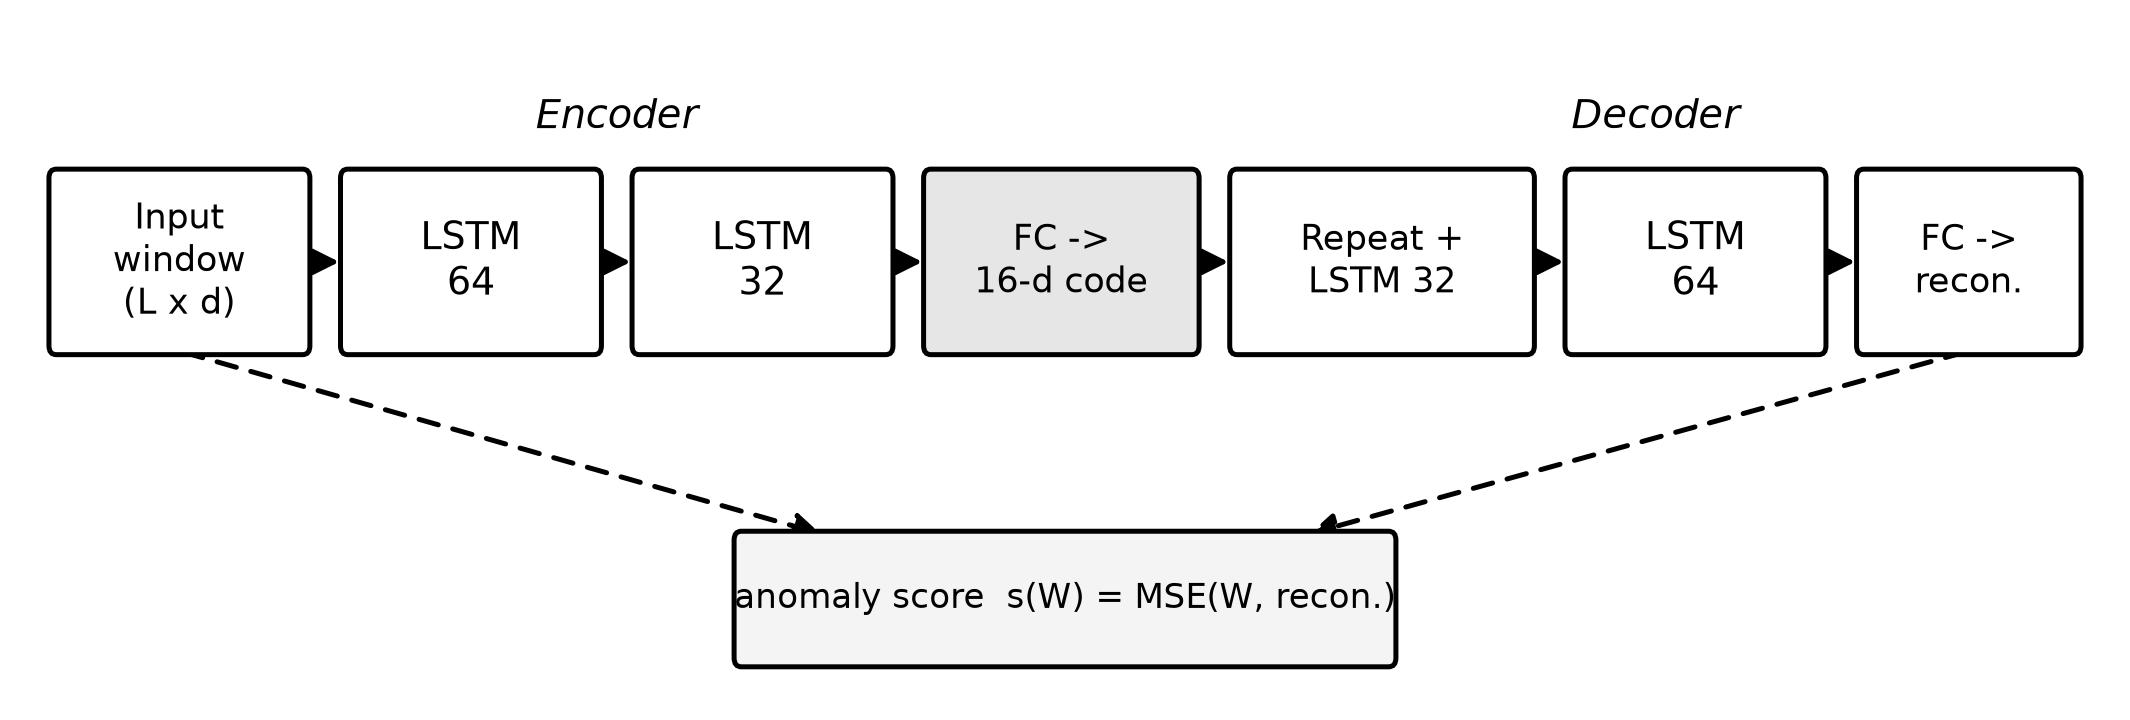
\includegraphics[width=\columnwidth]{figures/fig1_lstm_ae.png}
\caption{LSTM autoencoder architecture. A length-$L$ window is compressed to
a 16-dimensional code and reconstructed; reconstruction error is the anomaly
score.}
\label{fig:lstmae}
\end{figure}

Fig.~\ref{fig:lstmae} traces the shape of the data through the network. A
window enters as a 30-by-$d$ array. The encoder reads it with two stacked
LSTM layers of 64 and 32 units and keeps only the final hidden state of the
second layer, a 32-number summary of the whole window. A linear layer
compresses that to the 16-number code. The decoder reverses the path: it
repeats the code across all 30 timesteps, passes it through two LSTM layers
of 32 and 64 units, and maps the result back to a 30-by-$d$ reconstruction
with a final linear layer. Training pulls this reconstruction toward the
input on normal data, so a large error at test time marks an anomaly.
% R3: more detailed discussion of Fig. 1
The 16-dimensional bottleneck, shaded in Fig.~\ref{fig:lstmae}, is
deliberately narrower than both the input and the encoder output, which
forces the network to retain only the dominant temporal patterns of normal
operation; behaviour absent from the training data cannot be compressed
faithfully and therefore produces a large reconstruction error. Repeating
the code across all 30 timesteps gives the decoder the same summary at every
step, so the reconstruction depends on the learned representation rather
than on copying the input. The dashed arrows in the figure indicate that the
anomaly score compares the original window with this reconstruction, as
in (\ref{eq:score}).

% R3: motivation for the LSTM autoencoder
\textit{Choice of architecture.} The LSTM autoencoder is selected for four
reasons. First, recurrent units process a window in temporal order, which
suits faults and attacks whose signatures develop gradually across
timesteps. Second, the model is compact, which keeps the repeated
inner-loop updates of meta-training inexpensive and numerically stable.
Third, attention-based encoders typically require substantially more
training data, and with a support set of only a few dozen windows they are
prone to overfitting. Fourth, the LSTM encoder-decoder of Malhotra et
al.~\cite{malhotra2016} is a widely used baseline for multi-sensor anomaly
detection; adopting it isolates the contribution of meta-learning from that
of architectural novelty. Because MAML is model-agnostic, the procedure
applies unchanged to GRU, temporal convolutional, or Transformer encoders,
which are left for future work.

\subsection{Meta-Training and a Verification Worth Adopting}
\label{sec:verify}

MAML looks for an initialization from which a few gradient steps on a
task's support set produce well-adapted parameters~\cite{finn2017}. We use
the first-order variant~\cite{antoniou2019}, which drops the second-order
term to save cost while staying close to full MAML in practice. At each
outer step we sample a batch of tasks. For task $i$ we copy the current
model and adapt the copy on that task's support set $S_i$; one inner step is
shown in (\ref{eq:inner}), and it repeats $m$ times.
\begin{equation}
\theta_i' = \theta - \alpha \nabla_{\theta}\mathcal{L}(\theta; S_i)
\label{eq:inner}
\end{equation}
The adapted copy is written with a prime, $\alpha$ is the inner-loop
learning rate, and the loss is the mean reconstruction error of
(\ref{eq:score}) over the given set. The meta-model is then updated from the
query loss of each adapted copy, as in (\ref{eq:outer}), where $\beta$ is
the outer-loop learning rate, $B$ is the number of tasks in the batch, and
$Q_i$ is task $i$'s query set.
\begin{equation}
\theta \leftarrow \theta - \frac{\beta}{B}\sum_{i=1}^{B}
\nabla_{\theta_i'}\mathcal{L}(\theta_i'; Q_i)
\label{eq:outer}
\end{equation}
The step that matters is where the gradient in (\ref{eq:outer}) is taken. It
is computed with respect to the adapted copy and then written onto the
shared parameters before the optimizer moves them. This transfer is exactly
the line that is easy to drop. If the query loss is computed on the copy but
the backward pass and optimizer step are applied to the original model
instead, the gradient never reaches the shared parameters, because the copy
is a detached set of leaf tensors. Training then runs without training
anything: a loss prints, a validation curve appears, and checkpoints save,
while the meta-model stays at its initialization.

Algorithm~\ref{alg:fomaml} states the corrected procedure end to end.
Line~11 is the transfer just described: the averaged query gradient is
placed onto the shared parameters before the optimizer step, and omitting it
is what silently freezes the meta-model. We write the per-task adapted copy
as $\theta'$, matching (\ref{eq:inner}) and (\ref{eq:outer}).

\begin{algorithm}[t]
\caption{Corrected First-Order MAML Meta-Training}
\label{alg:fomaml}
\begin{algorithmic}[1]
\Require tasks $\mathcal{T}$; rates $\alpha,\beta$; inner steps $m$; batch
size $B$; outer steps $N$
\Ensure meta-initialization $\theta^{*}$
\State init $\theta$; \ $\mathrm{opt}\gets\mathrm{Adam}(\theta,\ \mathrm{lr}{=}\beta)$
\For{$\mathrm{step}=1$ \textbf{to} $N$}
  \State sample $B$ tasks from $\mathcal{T}$; \ $g\gets 0$
  \For{each task $\mathcal{T}_i$ (support $S_i$, query $Q_i$)}
    \State $\theta'\gets\mathrm{copy}(\theta)$
    \For{$j=1$ \textbf{to} $m$}
      \State $\theta'\gets\theta'-\alpha\nabla\mathcal{L}(\theta';S_i)$
    \EndFor
    \State $g\gets g+\nabla\mathcal{L}(\theta';Q_i)$ \Comment{w.r.t.\ $\theta'$}
  \EndFor
  \State $\theta.\mathrm{grad}\gets g/B$ \Comment{transfer step}
  \State $\mathrm{clip\_grad\_norm}(\theta,1.0)$; \ $\mathrm{opt.step}()$
\EndFor
\State \Return $\theta^{*}$
\end{algorithmic}
\end{algorithm}

We caught this in our own early implementation and now treat three checks
as mandatory before trusting any first-order MAML run:
\begin{enumerate}
\item After a single outer step, confirm that every meta-parameter's
gradient attribute is populated, not empty.
\item Snapshot the meta-parameters before and after a step and confirm they
changed. A gradient that exists but is never applied is just as broken as
one that never arrives.
\item Watch the shape of the meta-validation loss. A curve that is flat from
the very first evaluation and never moves, however long training runs, is
not evidence of a fast-converging problem. It is the signature of a
meta-model stuck at its initialization, and it looks enough like
convergence to pass casual inspection.
\end{enumerate}
Every result in this paper comes from a run that passes all three checks,
so the reported meta-model provably trains.

\subsection{Transferring Between Plants}

SWaT and WADI have 51 and 123 sensors respectively, with no correspondence
between them, so a model trained on one cannot be applied to the other
without a bridge. We fit Principal Component Analysis~\cite{jolliffe2016} on
each plant's own normal data separately and keep the first 32 components,
scaled to the unit range using that plant's normal statistics. Thirty-two
components retain 99.99 percent of SWaT's variance and 97.33 percent of
WADI's, so the loss from the projection itself is small. The two
32-dimensional spaces are not aligned with each other in any semantic sense;
what can transfer between them is temporal reconstruction structure, not a
shared sensor meaning.

\begin{figure}[t]
\centering
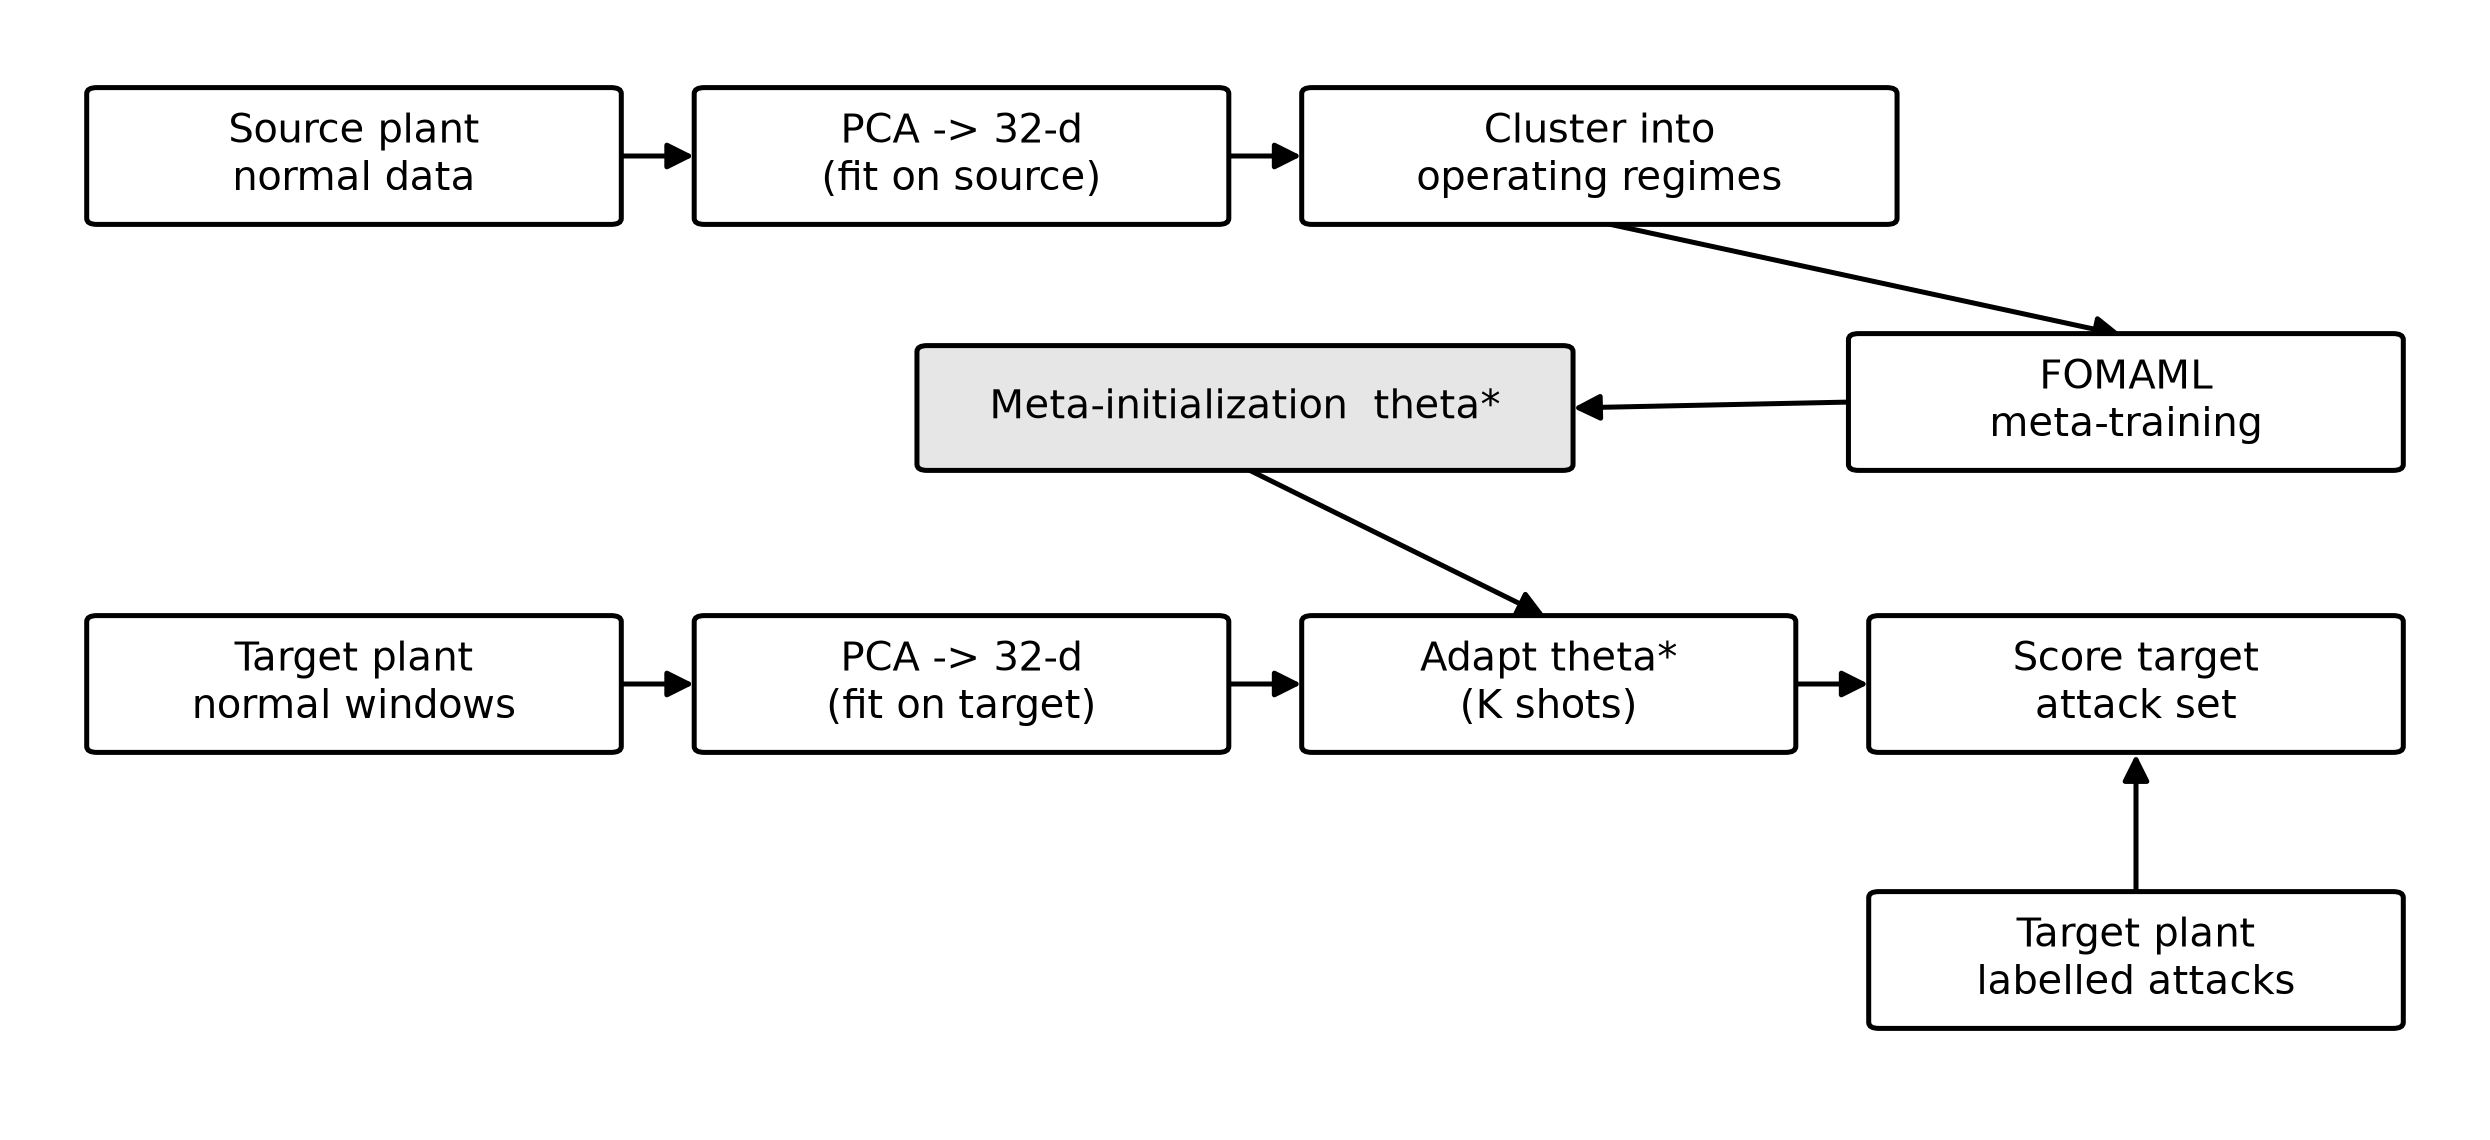
\includegraphics[width=\columnwidth]{figures/fig2_pipeline.png}
\caption{Cross-plant transfer pipeline. Each plant is projected to a common
32-d PCA space; the model is meta-trained on the source plant's regimes,
then adapted on a few target-plant normal windows before scoring the target
attack set.}
\label{fig:pipeline}
\end{figure}

Meta-training happens on the source plant. We split its normal operation
into behavioural regimes by clustering windows on their per-feature mean and
standard deviation, and treat each regime as a meta-learning task, following
the same episodic setup as~\cite{finn2017}.
% R3: box-by-box walk-through of Fig. 2
Fig.~\ref{fig:pipeline} lays out the full pipeline in two rows. The upper
row operates on the source plant only. Its normal data are first projected
to 32 dimensions by a PCA fitted on that plant; the projected windows are
then clustered into operating regimes; and FOMAML treats each regime as a
separate task to produce the meta-initialization $\theta^{*}$, shaded in the
centre of the figure. The lower row operates on the target plant. Its normal
windows are projected by a PCA fitted independently on the target's own
normal data, so no sensor correspondence between the plants is required. A
support set of $K$ projected windows adapts $\theta^{*}$ through the
inner-loop update of (\ref{eq:inner}), and the adapted model then scores the
target plant's labelled attack set, whose labels are used only to compute
ROC-AUC. The only arrow linking the two rows carries model parameters; no
raw data, sensor mapping, or anomaly label crosses between the plants.

\subsection{Label-Free Thresholding}

Detection needs a threshold, and we set it without any anomaly label, from
the reconstruction errors on the support windows alone. With more than one
support window the threshold is given by (\ref{eq:thresh}), where the mean
and standard deviation are taken over the support-window errors.
\begin{equation}
\tau = \mu_S + 2\sigma_S
\label{eq:thresh}
\end{equation}
With a single support window no standard deviation exists, so the threshold
falls back to 1.20 times the mean error, which keeps false positives in
check under the tightest label scarcity. A test window is flagged when its
score from (\ref{eq:score}) exceeds the threshold. Because the threshold
draws only on support-window errors, no anomaly label enters at any point.

\section{Experimental Setup}
\label{sec:setup}

SWaT is a six-stage water treatment process instrumented with 51 sensors and
actuators. WADI is a water distribution network with 123 channels. Both
provide a normal operating recording and a separate, labelled attack
recording. Cleaning both streams needed some care that is easy to get wrong
quietly: SWaT's attack label contains a typo variant of the word that a
naive string match on the correct spelling misses, silently dropping real
attack rows, and WADI's label column uses an inverted convention where a
negative value marks an attack. Both streams are downsampled by a factor of
ten and scaled with a MinMax transform fitted on the normal recording only,
then applied to both recordings with clipping to keep test-time values in
range. Table~\ref{tab:hyper} lists the main hyperparameters and
Table~\ref{tab:testbeds} summarizes the two testbeds after this processing.

\begin{table}[t]
\caption{Main Hyperparameters}
\label{tab:hyper}
\centering
\footnotesize
\begin{tabular}{@{}ll@{}}
\toprule
Hyperparameter & Value \\
\midrule
Window length $L$ & 30 \\
Encoder hidden units & 64, 32 \\
Bottleneck dimension & 16 \\
Inner-loop learning rate ($\alpha$) & 0.01 \\
Outer-loop learning rate ($\beta$) & 0.001 \\
Inner-loop steps ($m$) & 10 \\
Tasks per outer step ($B$) & 4 \\
Outer steps (max) & 5000 \\
Support sizes tested ($K$) & 20, 50, 100 \\
Training seeds & 6 \\
PCA projection dimension & 32 \\
\bottomrule
\end{tabular}
\end{table}

\begin{table}[t]
\caption{Testbed Summary After Preprocessing}
\label{tab:testbeds}
\centering
\footnotesize
\begin{tabular}{@{}lrr@{}}
\toprule
Property & SWaT & WADI \\
\midrule
Sensors / actuators & 51 & 123 \\
Normal windows & 4,948 & 7,843 \\
Attack windows & 4,497 & 1,726 \\
Anomalous windows & 648 & 140 \\
\bottomrule
\end{tabular}
\end{table}

We compare three methods at the transfer task. MAML-transfer is the
meta-trained model of Section~III, adapted on a support set of target-plant
normal windows. Static-transfer is the same architecture trained
conventionally on the source plant's full normal data, then adapted on the
same target support set, which isolates whatever meta-learning adds over
ordinary pre-training.
% R1: name the conventional transfer-learning baseline explicitly
Static-transfer is therefore the conventional transfer-learning baseline:
pre-training on the source plant followed by fine-tuning on the target,
with the architecture, projection, support set, and adaptation budget held
identical to MAML-transfer so that the two differ only in how the source
model is trained.
Target-static is a reference model trained directly on the target plant,
standing in for the best case an operator could reach with unlimited
target-plant data. We test support sizes of 20, 50, and 100 normal windows;
across this range ROC-AUC shifts by less than a point in every case, so the
seeded comparison fixes the support set at 50 windows. To check whether
meta-learning's edge over static pre-training, if any, survives beyond a
single lucky run, we repeat the full training procedure, both the
meta-learned and the static model, across six independent training seeds at
that support size and run a paired statistical test on the per-seed ROC-AUC
difference. Meta-training uses early stopping on the meta-validation loss,
evaluated every 250 outer steps with a patience of six, so the 5,000 outer
steps in Table~\ref{tab:hyper} is an upper bound rather than a fixed count.

Within a single plant, before testing transfer, we also checked whether
meta-learning helps at all against a properly trained static autoencoder on
SWaT and WADI individually. It does not: meta-learning never clears a
properly trained static autoencoder on either testbed, so we do not repeat
those tables here; the full within-plant evaluation, across three benchmarks
including NASA's SMAP telemetry set, is reported in a separate manuscript
under preparation. That null result is what pushed us toward testing
transfer specifically, since within a single plant the operating conditions
are too alike for adaptation to have much to work with.

\section{Results}

\begin{table}[t]
\caption{Cross-Plant Transfer, Mean ROC-AUC Over Six Training Seeds
($K=50$)}
\label{tab:results}
\centering
\footnotesize
\begin{tabular}{@{}lccc@{}}
\toprule
Direction & Target-static & MAML-transfer & Static-transfer \\
\midrule
WADI to SWaT & 0.812 & 0.796 & 0.797 \\
SWaT to WADI & 0.707 & 0.574 & 0.595 \\
\bottomrule
\end{tabular}
\end{table}

Table~\ref{tab:results} gives the transfer result in both directions. Moving
a model meta-trained on WADI into SWaT works well. Across six seeds,
MAML-transfer reaches a mean ROC-AUC of 0.796, and Static-transfer reaches
0.797, both close to the 0.812 achieved by training directly on SWaT. The
paired difference between MAML-transfer and Static-transfer is $-0.001$,
with a 95 percent confidence interval of $[-0.025, +0.024]$, so
meta-learning is not distinguishable from conventional pre-training here.
Moving the other way, from SWaT into WADI, both transfer methods fall
further short of the 0.707 reached by training directly on WADI, and the
same statistical parity holds between MAML-transfer and Static-transfer.

The number worth taking away from this table is not the comparison between
the two transfer methods, which come out level. It is that WADI-to-SWaT
transfer at 0.796 sits within two points of the 0.812 an operator would get
by collecting enough SWaT data to train on directly. For a plant that has
only a handful of normal windows and no attack history, reaching most of the
way to the fully-trained number without either is a real capability,
whether the model that gets you there was meta-trained or just
conventionally pre-trained on a different plant.

The asymmetry between the two directions is consistent with how much
internal variety each plant's own normal operation has, and the
principal-component spectra of the normal data quantify the difference. In
SWaT the first component accounts for 48.84 percent of the variance and the
first five for 90.43 percent, so the variation is dominated by a few strong,
well-separated modes, consistent with a process that cycles through its six
treatment stages. In WADI the first component accounts for only 29.37
percent and the first five for 68.08 percent, with ten needed to reach 81.99
percent, so the variance is spread thinly with no dominant mode, the
signature of normal operation that stays close to a single behavioural
regime. A model transferring into a target with some internal structure of
its own has more to align to than one transferring into a near-uniform
target, and that pattern matches what Table~\ref{tab:results} shows.

\section{Discussion}

The practical reading of this result is straightforward. If a new plant is
similar enough in kind to an existing, well-instrumented one, and especially
if that plant's own operation is not perfectly uniform, a source-trained
detector adapted on a small support set of the new plant's normal data can
substitute for months of data collection. That holds whether the
source-trained detector was produced by meta-learning or by ordinary
training, which matters for anyone deciding whether the extra machinery of
meta-learning is worth adopting. On this evidence, the answer is that the
transfer capability, not the meta-learning method specifically, is what does
the work.

The verification checks in Section~\ref{sec:verify} are worth carrying into
any project using first-order MAML, not just this one. A silent training
failure that still produces a plausible-looking loss curve is the kind of
bug that survives code review and gets noticed, if at all, only when someone
questions why a supposedly meta-learned model behaves exactly like an
untrained one.

\section{Limitations}

The transfer result rests on a PCA bridge between two sensor spaces that
share no semantic correspondence, and the asymmetry between directions could
partly reflect how much each plant's structure survives the projection,
though the target-static reference uses the same projection and still
reaches a reasonable number on WADI, so the bridge is not the whole
explanation. Six training seeds are enough to say that a small edge for
meta-learning over static pre-training does not hold up, but not enough to
certify the two methods as exactly equal. The result is specific to
reconstruction-based detection and to these two testbeds; whether it
generalizes to other plant pairs or other anomaly-scoring approaches is
untested here.
% R1: limitation of using only two testbeds
The evaluation is further limited to two testbeds. SWaT and WADI are both
water systems developed by the same research centre and share similar
PLC-based control architectures, so the transfer demonstrated here is
between related cyber-physical systems rather than between fundamentally
different industrial domains. Whether the result holds for transfer across
domains, for example from water treatment to power distribution or
manufacturing, and for a larger number of source plants, remains to be
established on additional industrial testbeds.

\section{Conclusion}

We set out to check whether a meta-learned anomaly detector can be handed to
a new industrial plant with almost no data of its own and still work. Once a
silent implementation failure common to first-order MAML is caught and
fixed, the answer is a qualified yes. Cross-plant transfer between two real
water-treatment testbeds nearly reaches the performance of training directly
on the target plant, which is a genuinely useful capability for deployment.
Meta-learning itself does not clearly beat conventional pre-training at this
task, tested across independent training seeds in both directions, so the
practical recommendation is to use whichever pre-training approach is
convenient and to invest the effort instead in checking, with the three
tests we describe, that the training actually happened.
% R1 / R3: future work
Future work will extend the evaluation to industrial testbeds from other
domains and to alternative sequence encoders.

\IEEEtriggeratref{9}
\begin{thebibliography}{99}

\bibitem{cook2020} A.~A. Cook, G.~M{\i}s{\i}rl{\i}, and Z.~Fan, ``Anomaly
detection for IoT time-series data: A survey,'' \textit{IEEE Internet Things
J.}, vol.~7, no.~7, pp.~6481--6494, 2020.

\bibitem{hospedales2022} T.~M. Hospedales, A.~Antoniou, P.~Micaelli, and
A.~J. Storkey, ``Meta-learning in neural networks: A survey,'' \textit{IEEE
Trans. Pattern Anal. Mach. Intell.}, vol.~44, no.~9, pp.~5149--5169, 2022.

\bibitem{finn2017} C.~Finn, P.~Abbeel, and S.~Levine, ``Model-agnostic
meta-learning for fast adaptation of deep networks,'' in \textit{Proc. 34th
Int. Conf. Mach. Learn.}, Sydney, Australia, 2017, pp.~1126--1135.

\bibitem{malhotra2016} P.~Malhotra, A.~Ramakrishnan, G.~Anand, L.~Vig,
P.~Agarwal, and G.~Shroff, ``LSTM-based encoder-decoder for multi-sensor
anomaly detection,'' in \textit{Proc. ICML Anomaly Detection Workshop}, New
York, USA, 2016, arXiv:1607.00148.

\bibitem{mathur2016} A.~P. Mathur and N.~O. Tippenhauer, ``SWaT: A water
treatment testbed for research and training on ICS security,'' in
\textit{Proc. Int. Workshop Cyber-Physical Syst. Smart Water Netw.}, Vienna,
Austria, 2016, pp.~31--36.

\bibitem{ahmed2017} C.~M. Ahmed, V.~R. Palleti, and A.~P. Mathur, ``WADI: A
water distribution testbed for research in the design of secure cyber
physical systems,'' in \textit{Proc. 3rd Int. Workshop Cyber-Physical Syst.
Smart Water Netw.}, Pittsburgh, USA, 2017, pp.~25--28.

\bibitem{pang2021} G.~Pang, C.~Shen, L.~Cao, and A.~van~den Hengel, ``Deep
learning for anomaly detection: A review,'' \textit{ACM Comput. Surv.},
vol.~54, no.~2, pp.~1--38, 2021.

\bibitem{deng2021} A.~Deng and B.~Hooi, ``Graph neural network-based anomaly
detection in multivariate time series,'' in \textit{Proc. AAAI Conf. Artif.
Intell.}, 2021, vol.~35, pp.~4027--4035.

\bibitem{chen2022} Z.~Chen, D.~Chen, X.~Zhang, Z.~Yuan, and X.~Cheng,
``Learning graph structures with transformer for multivariate time series
anomaly detection in IoT,'' \textit{IEEE Internet Things J.}, vol.~9,
no.~12, pp.~9179--9189, 2022.

\bibitem{correia2024} L.~Correia, J.~C. Goos, P.~Klein, T.~B{\"a}ck, and
A.~V. Kononova, ``Online model-based anomaly detection in multivariate time
series: Taxonomy, survey, research challenges and future directions,''
\textit{Eng. Appl. Artif. Intell.}, vol.~138, p.~109323, 2024.

% R1: new references -- verify details against the publisher pages
\bibitem{audibert2020} J.~Audibert, P.~Michiardi, F.~Guyard, S.~Marti, and
M.~A. Zuluaga, ``USAD: Unsupervised anomaly detection on multivariate time
series,'' in \textit{Proc. 26th ACM SIGKDD Int. Conf. Knowl. Discov. Data
Min.}, 2020, pp.~3395--3404.

\bibitem{tuli2022} S.~Tuli, G.~Casale, and N.~R. Jennings, ``TranAD: Deep
transformer networks for anomaly detection in multivariate time series
data,'' \textit{Proc. VLDB Endow.}, vol.~15, no.~6, pp.~1201--1214, 2022.

\bibitem{antoniou2019} A.~Antoniou, H.~Edwards, and A.~Storkey, ``How to
train your MAML,'' in \textit{Proc. 7th Int. Conf. Learn. Represent.}, New
Orleans, USA, 2019, arXiv:1810.09502.

\bibitem{li2017} Z.~Li, F.~Zhou, F.~Chen, and H.~Li, ``Meta-SGD: Learning to
learn quickly for few-shot learning,'' arXiv:1707.09835, 2017.

\bibitem{moon2023} J.~Moon, Y.~Noh, S.~Jung, J.~Lee, and E.~Hwang, ``Anomaly
detection using a model-agnostic meta-learning-based variational
auto-encoder for facility management,'' \textit{J. Build. Eng.}, vol.~68,
p.~106099, 2023.

\bibitem{zhang2021} S.~Zhang, F.~Ye, B.~Wang, and T.~G. Habetler, ``Few-shot
bearing fault diagnosis based on model-agnostic meta-learning,''
\textit{IEEE Trans. Ind. Appl.}, vol.~57, no.~5, pp.~4754--4764, 2021.

\bibitem{jolliffe2016} I.~T. Jolliffe and J.~Cadima, ``Principal component
analysis: A review and recent developments,'' \textit{Philos. Trans. R. Soc.
A}, vol.~374, no.~2065, p.~20150202, 2016.

\end{thebibliography}

\end{document}
